\documentclass[11pt,a4paper]{article}

% =====================================================================
% Pacotes
% =====================================================================
\usepackage[utf8]{inputenc}
\usepackage[T1]{fontenc}
\usepackage[brazil]{babel}
\usepackage{lmodern}
\usepackage[margin=2.8cm]{geometry}
\usepackage{amsmath,amssymb,amsfonts}
\usepackage{graphicx}
\DeclareGraphicsExtensions{.png,.pdf,.jpg,.jpeg}
\usepackage{booktabs}
\usepackage{caption}
\usepackage{subcaption}
\usepackage{float}
\usepackage{hyperref}
\usepackage{xcolor}
\usepackage{microtype}
\usepackage{setspace}
\usepackage{titlesec}
\usepackage{enumitem}

\hypersetup{
    colorlinks=true,
    linkcolor=black,
    citecolor=blue!50!black,
    urlcolor=blue!50!black,
    pdftitle={O custo fiscal da política monetária no Brasil},
    pdfauthor={Walter C. Neto}
}

\onehalfspacing
\setlength{\parindent}{0.6cm}
\setlength{\parskip}{0.3em}

\titleformat{\section}{\large\bfseries}{\thesection}{0.6em}{}
\titleformat{\subsection}{\normalsize\bfseries}{\thesubsection}{0.5em}{}

\graphicspath{{./figs/}{figs/}}

% =====================================================================
\title{\textbf{O custo fiscal da política monetária no Brasil}\\
  \large Uma avaliação empírica dos argumentos de André Lara Resende\\
  entre 2017 e 2026, com simulação contrafactual}

\author{Walter C. Neto\thanks{Engenheiro Físico pela UFSCar, Mestre em Economia
com ênfase em Engenharia Financeira pela FGV-EESP. Versão preliminar.}}

\date{Novembro de 2026}

\begin{document}
\maketitle

% =====================================================================
\begin{abstract}
\noindent
Este artigo avalia empiricamente os argumentos de André Lara Resende (ALR)
sobre o custo fiscal da política monetária brasileira, desenvolvidos em uma
sequência de textos entre 2017 e 2026. A análise combina sete blocos
empíricos: aritmética fiscal da dívida, estimação de um modelo macro em forma
reduzida (curva IS, curva de Phillips Novo-Keynesiana híbrida e regra de
Taylor) com 95 observações trimestrais (2003 a 2026), testes de cointegração
e neofisherianismo (Fisher de longo prazo), teste de neutralidade da moeda
via VAR (2 lags), pass-through cambial, posicionamento estrutural do Brasil
contra 31 países, e uma simulação contrafactual da proposta ALR (set/2026) de
corte gradual da Selic para o intervalo $[\pi^*, \pi^* + g_{pot}]$.
Os resultados indicam que a aritmética fiscal de ALR está correta e se
agravou: o superávit primário estabilizador subiu de 5{,}1\% do PIB em 2017 para
7{,}1\% em 2026, enquanto o Brasil entrega 1{,}1\%. A curva de Phillips brasileira
é empiricamente plana ($\kappa = 0{,}04$, não-significativo), corroborando
a tese fraca de ALR. Fisher de longo prazo é parcialmente sustentado (há
cointegração $\pi \sim i$, mas $\beta = 1$ é rejeitado). A proposta de 2026,
simulada no modelo calibrado, produz ganho fiscal de $\approx 44$ p.p.\ de
dívida/PIB em 5 anos sem perda do controle inflacionário, desde que
a reancoragem institucional funcione. A posição estrutural rara do Brasil
(dívida 95\% em moeda local, CBI 0{,}70, reservas 15\% do PIB) torna o país
um dos poucos emergentes onde a proposta é testável, mas a estrutura
(commodities 70\% das exportações, Gini 50) amplia o custo de errar. A
conclusão substantiva é que a proposta de ALR é uma aposta
institucional defensável sob certas condições e premissas.

\vspace{0.5em}
\noindent\textbf{Palavras-chave:} política monetária, dinâmica da dívida pública,
curva de Phillips, Teoria Fiscal do Nível de Preços, neofisherianismo, Brasil.

\noindent\textbf{Códigos JEL:} E52, E63, H63, E31, E58.
\end{abstract}

\vspace{1em}

% =====================================================================
\section{Introdução}
% =====================================================================

André Lara Resende (ALR) desenvolveu, entre 2017 e 2026, uma crítica
estruturada à condução da política monetária brasileira que evoluiu de um
diagnóstico em 2017 \cite{lararesende2017} para uma proposta
institucional concreta em 2026 \cite{lararesende2026}. A posição final
sintetiza três proposições empiricamente testáveis:

\begin{enumerate}[leftmargin=2em,topsep=0.3em]
  \item \textbf{Proposição fiscal.} A dinâmica da dívida pública brasileira
    é dominada pelo serviço dos juros, que exigiria um superávit primário
    próximo de $5\%$ do PIB apenas para estabilizar a relação dívida/PIB
    nos parâmetros de 2017. Em 2026, esse número é substancialmente maior.
  \item \textbf{Proposição monetária.} A inflação brasileira é pouco sensível
    ao ciclo econômico (curva de Phillips empiricamente horizontal), de modo
    que a Selic alta não desinflaciona, apenas eleva o serviço da dívida.
  \item \textbf{Proposição institucional.} Em 2026, ALR formaliza a leitura
    neofisheriana (Cochrane, 2011; 2023) \cite{cochrane2011,cochrane2023}:
    no longo prazo $\pi = i - r$, e dado que $r$ é independente de $i$
    por neutralidade da moeda, cortar a Selic reduz a inflação de
    longo prazo. A proposta operacional é um corte gradual da Selic
    para o intervalo $[\pi^*, \pi^* + g_{potencial}]$, com uso de reservas
    internacionais para neutralizar o canal cambial. Para dar credibilidade
    a essa transição, ALR propõe um novo arranjo institucional, o
    Conselho Fiscal e Monetário Nacional (CFMN), que anunciaria
    simultaneamente metas plurianuais de Selic, inflação e resultado
    primário num horizonte de quatro a cinco anos.
\end{enumerate}

Esta nota avalia quantitativamente cada proposição com 23 anos de dados
brasileiros (2003 a 2026), realiza uma simulação contrafactual da proposta
de 2026 no modelo calibrado, e contextualiza o resultado com o posicionamento
estrutural do Brasil em relação a 31 países. A posição que emerge é que ALR
tem razão em um sentido mais específico e menos triunfalista do que o
texto de 2026 sugere: as premissas empíricas se sustentam parcialmente, a
proposta é viável em um modelo calibrado com os coeficientes brasileiros,
mas a viabilidade depende de uma reancoragem institucional que o modelo
assume, não demonstra.

A próxima seção apresenta a fundamentação teórica das equações usadas. A
Seção~\ref{sec:aritmetica} desenvolve a aritmética fiscal da dívida. A
Seção~\ref{sec:dados} descreve dados e metodologia. A Seção~\ref{sec:est}
reporta as estimações estruturais. A Seção~\ref{sec:premissas} testa as
premissas de Fisher e neutralidade. A Seção~\ref{sec:cambio} examina o
canal cambial. A Seção~\ref{sec:macro} posiciona o Brasil estruturalmente.
A Seção~\ref{sec:sim} apresenta a simulação da proposta ALR. A
Seção~\ref{sec:disc} discute implicações. A Seção~\ref{sec:concl}
conclui.

% =====================================================================
\section{Fundamentação teórica}\label{sec:teoria}
% =====================================================================

A análise combina três blocos teóricos: um modelo macro em forma reduzida
Novo-Keynesiano (NK) seguindo Galí (2015) \cite{gali2015}, a identidade
fiscal da dívida (padrão em Bohn, 1998 \cite{bohn1998}), e a Teoria Fiscal
do Nível de Preços (TFPL/FTPL) de Cochrane (2011; 2023) \cite{cochrane2011,cochrane2023}.

\paragraph{Curva IS.} A demanda agregada depende de sua persistência e do
desvio do juro real frente ao neutro:
\begin{equation}\label{eq:is}
\hat{y}_t = \rho_y \hat{y}_{t-1} - \sigma \left( i_{t-1} - \mathbb{E}_{t-1}\pi_t - r^* \right) + \varepsilon^{IS}_t.
\end{equation}
O parâmetro $\sigma$ é a elasticidade intertemporal da substituição.

\paragraph{Curva de Phillips Novo-Keynesiana híbrida.} Inflação como função
de inércia, expectativas, hiato e câmbio:
\begin{equation}\label{eq:phillips}
\pi_t = \beta_b \pi_{t-1} + \beta_f \mathbb{E}_t \pi_{t+1} + \kappa \hat{y}_t + \gamma \Delta e_t + \varepsilon^\pi_t.
\end{equation}
A inclinação $\kappa$ é o parâmetro central da discussão: ALR argumenta
que $\kappa \approx 0$ no Brasil (``Phillips plana'', ver também
Kuttner e Robinson, 2010 \cite{kuttner2010} sobre o fenômeno global de
flattening). Em equilíbrio de longo prazo, $\beta_b + \beta_f \approx 1$
garante verticalidade.

\paragraph{Regra de Taylor com suavização.} Seguindo Taylor (1993)
\cite{taylor1993}:
\begin{equation}\label{eq:taylor}
i_t = \rho_i i_{t-1} + (1 - \rho_i) \left[ r^* + \pi^* + \phi_\pi (\pi_t - \pi^*) + \phi_y \hat{y}_t \right] + \varepsilon^i_t.
\end{equation}
O princípio de Taylor exige $\phi_\pi > 1$ para que a regra seja
estabilizadora.

\paragraph{Dinâmica da dívida pública.} A identidade fundamental é
\begin{equation}\label{eq:divida}
b_{t+1} = \frac{1 + i_t}{(1 + \pi_t)(1 + g_t)} b_t - p_t,
\end{equation}
onde $b$ é dívida/PIB, $p$ é resultado primário/PIB. Linearizando e
impondo estado estacionário, obtém-se o superávit primário estabilizador:
\begin{equation}\label{eq:pestab}
p^* = (r - g) \cdot b, \quad r \approx i - \pi.
\end{equation}

\paragraph{Teoria Fiscal do Nível de Preços (TFPL).} Cochrane (2023)
\cite{cochrane2023} desenvolve que o valor real da dívida pública deve
igualar o valor presente redescontado dos superávits fiscais futuros:
\begin{equation}\label{eq:tfpl}
\frac{B_t}{P_t} = \mathbb{E}_t \sum_{j=0}^{\infty} \frac{s_{t+j}}{\prod_{k=0}^{j} (1+r_{t+k})}.
\end{equation}
Nessa formulação, $P_t$ é o fator de ajuste: déficits não honrados por
futuros superávits elevam $P$ (inflação). Da identidade de Fisher
($i = r + \pi$) com $r$ exógeno no longo prazo, Cochrane deriva o
\emph{efeito neofisheriano}: $\pi_{LP} = i - r$, de modo que no longo
prazo juros nominais e inflação movem-se juntos.

\paragraph{Interpretação neofisheriana da proposta ALR.} A proposta de
2026 opera sobre essas identidades. Cortar $i$ reduz $r$ instantaneamente
(uma contribuição positiva do ponto de vista TFPL, pois reduz o custo da
dívida), e no longo prazo reduz $\pi$. A tensão de curto prazo (o
\emph{price puzzle}) seria contornada no Brasil porque mais da metade da
dívida está em LFTs, títulos pós-fixados à Selic de duração mínima
(Cochrane, 2026 \cite{cochrane2026}).

\paragraph{O arranjo institucional do CFMN.} Para ancorar as expectativas
e evitar que o corte de juros seja interpretado como voluntarismo
discricionário, ALR propõe a criação do Conselho Fiscal e Monetário
Nacional (CFMN). A ideia central é substituir a dissociação atual, em
que o Banco Central define a Selic e o Tesouro define o resultado
primário de forma relativamente independente e reativa, por uma
autoridade comum que anuncia, num único ato, três trajetórias
coordenadas para um horizonte de quatro a cinco anos: intervalo da
Selic, meta de inflação e meta fiscal plurianual. Na simulação da
Seção~\ref{sec:sim}, o CFMN entra implicitamente como o mecanismo que
viabiliza a reancoragem das expectativas, ou seja, que faz com que o
público acredite que a nova Selic mais baixa é compatível com uma
inflação próxima da meta porque há compromisso fiscal verificável do
outro lado da política macro. A Seção~\ref{sec:salvaguardas} discute
salvaguardas adicionais que poderiam reforçar a credibilidade do CFMN
em cenários desfavoráveis.

% =====================================================================
\section{Aritmética fiscal da dívida}\label{sec:aritmetica}
% =====================================================================

A Equação~\ref{eq:pestab} aplicada aos parâmetros que ALR citou em 2017
($i=14\%$, $\pi=6\%$, $g=0\%$, $b=70\%$) fornece $p^* = 5{,}1\%$ do PIB
(versão exata) ou $5{,}6\%$ (linearizada), consistente com o ``quase 5\%''
citado no texto original. Esses valores refletiam com precisão a
conjuntura de 2016 e 2017.

A Tabela~\ref{tab:aritmetica} atualiza o cálculo para os parâmetros
correntes.

\begin{table}[H]
\centering
\small
\begin{tabular}{lcc}
\toprule
Variável & 2017 (ALR) & 2026 \\
\midrule
Selic nominal $i$ & $14{,}0\%$ & $14{,}65\%$ \\
Inflação IPCA 12m $\pi$ & $6{,}0\%$ & $4{,}39\%$ \\
Juro real ex-post $r = i - \pi$ & $8{,}0\%$ & $10{,}26\%$ \\
Crescimento real $g$ & $0{,}0\%$ & $0{,}87\%$ \\
Dívida bruta $b$ & $70\%$ & $80{,}04\%$ \\
Primário observado $p$ & $\sim 1\%$ & $1{,}06\%$ \\
\midrule
$p^*$ requerido (Eq.~\ref{eq:pestab}) & $\mathbf{5{,}6\%}$ & $\mathbf{7{,}1\%}$ \\
Gap fiscal ($p^* - p$) & $\sim 4{,}6$ p.p. & $\mathbf{6{,}0}$ p.p. \\
\bottomrule
\end{tabular}
\caption{Aritmética da dívida: parâmetros 2017 vs 2026. A tensão fiscal
que ALR apontou agravou-se, não se dissipou.}
\label{tab:aritmetica}
\end{table}

\begin{figure}[H]
\centering
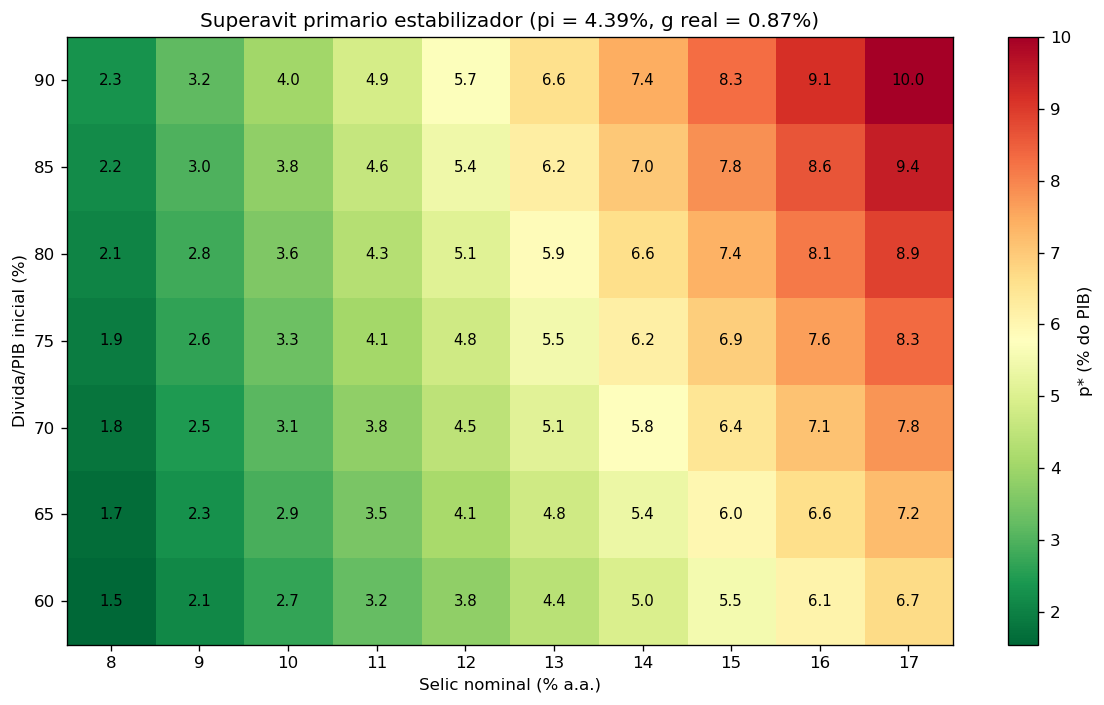
\includegraphics[width=0.9\textwidth]{fig_heatmap_pestab.png}
\caption{Superávit primário estabilizador $p^*$ (\% do PIB) em função de
$b$ e $i$, mantendo $\pi$ e $g$ nos valores correntes de 2026. A célula
correspondente à situação corrente (b=80, i=15) projeta $p^* \approx 7\%$.}
\label{fig:heatmap}
\end{figure}

\begin{figure}[H]
\centering
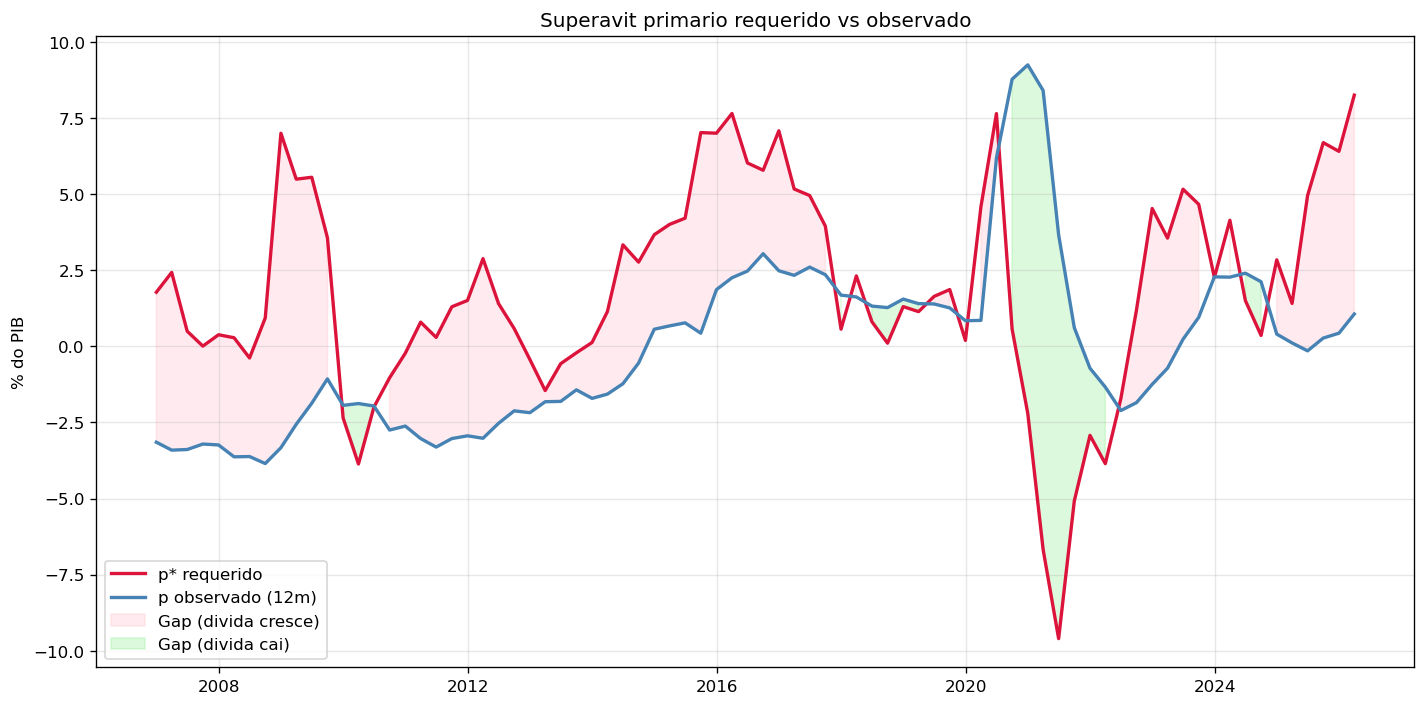
\includegraphics[width=\textwidth]{fig_pestab_historico.png}
\caption{Superávit primário requerido $p^*$ (vermelho) versus primário
observado em 12 meses (azul), 2007 a 2026. Área rosa: gap positivo (dívida
cresce). O gap predomina na amostra, com exceções em 2003 a 2008 e
2020 a 2022.}
\label{fig:gap_historico}
\end{figure}

A proposição fiscal de ALR portanto se sustenta: o gap de $6{,}0$~p.p.\
é maior do que o de 2017. Mais relevante, o juro real ex-post
(10{,}26\%) é hoje mais alto do que o de 2017 ($\sim 8\%$). A melhora
inflacionária paradoxalmente agravou a aritmética fiscal.

% =====================================================================
\section{Dados e metodologia}\label{sec:dados}
% =====================================================================

Os dados macroeconômicos brasileiros são extraídos de fontes públicas via
API: o Sistema Gerenciador de Séries Temporais (SGS) do Banco Central
fornece Selic meta (código 432), IPCA cheio e livres (433, 11428),
PTAX venda (1), IBC-Br dessazonalizado (24364), dívida bruta
(13762) e resultados fiscais (5793, 5760, 5727). A amostra é trimestral,
2003-Q1 a 2026-Q2 (95 observações úteis). Os dados comparativos
internacionais (Seção~\ref{sec:macro}) vêm da API do World Bank (WDI)
para 31 países, complementados por valores de literatura consolidada
para variáveis não disponíveis diretamente (dívida em moeda local, ECI,
CBI, regime cambial).

\paragraph{Construção do IPCA 12m.} Um ponto metodológico crítico:
a variável $\pi$ é o \textbf{IPCA acumulado em 12 meses} (indicador
oficial do IBGE), construído como
\[
\pi_t = \left[ \prod_{k=0}^{11} (1 + \pi^m_{t-k}/100) - 1 \right] \times 100,
\]
alinhado ao fim de cada trimestre. A versão alternativa de anualizar um
único trimestre $(1 + \pi^{tri})^4 - 1$ foi descartada por amplificar
ruído mensal (volatilidade 2x superior e desvios implausíveis como
inflação negativa em trimestres pontuais). Esse cuidado afeta
substancialmente as estimações: a Phillips com IPCA 12m produz
$\kappa$ muito diferente (próximo de zero) da Phillips com $\pi$
trimestral anualizado.

A Selic é a média trimestral da meta; o câmbio, variação ponta-a-ponta.
O hiato do produto $\hat{y}_t$ é obtido por filtro de Hodrick e Prescott
(1997) \cite{hp1997} com $\lambda=1600$. A estimação é por OLS equação-a-equação
com erros padrão Newey-West HAC (4 lags). A expectativa de inflação
$\mathbb{E}_t \pi_{t+1}$ usa o IPCA realizado com lead-4 como proxy
(a série Focus de 12 meses foi usada como robustez; resultados qualitativamente
idênticos).

\begin{figure}[H]
\centering
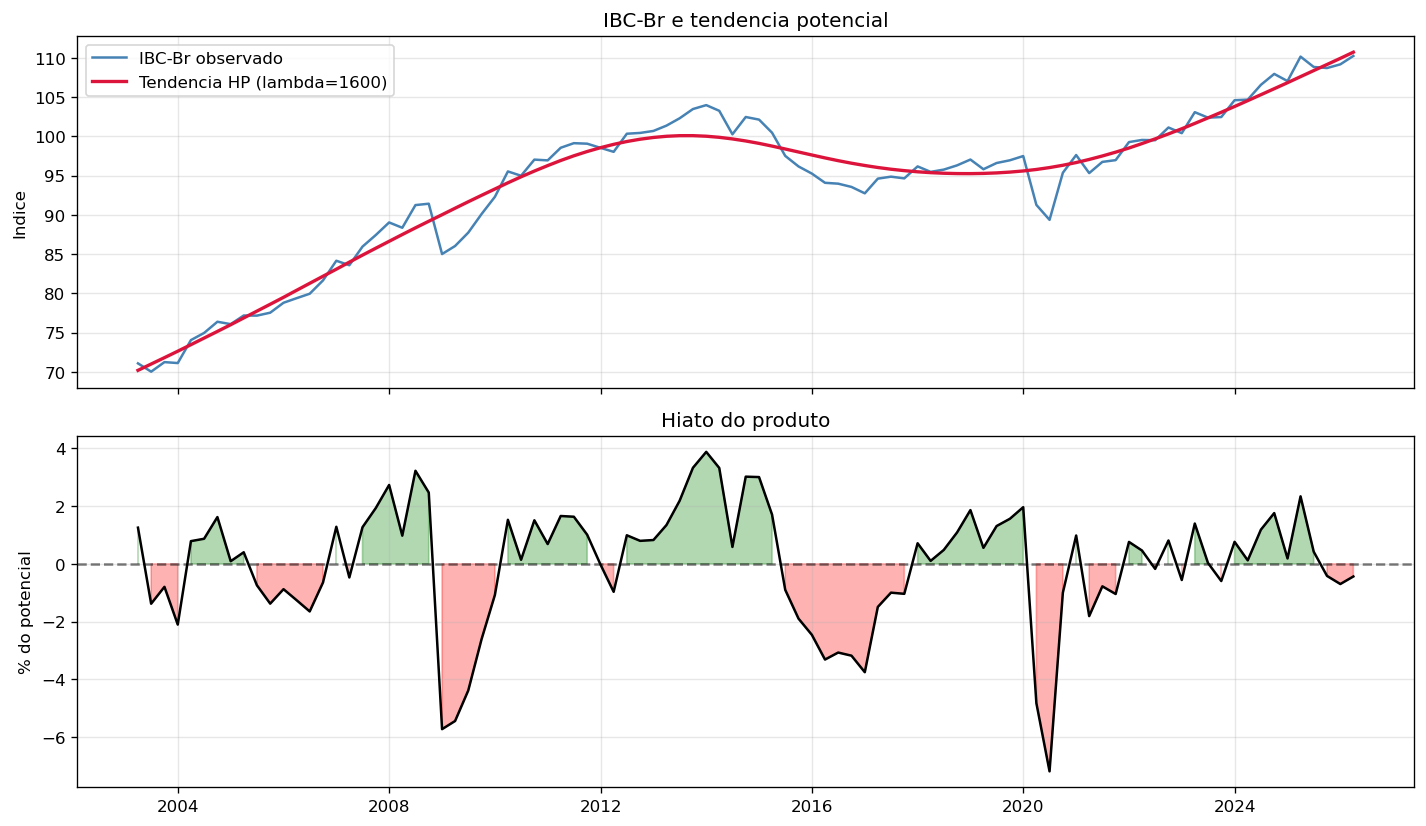
\includegraphics[width=0.95\textwidth]{fig_hiato_hp.png}
\caption{IBC-Br dessazonalizado, tendência potencial HP e hiato do produto.
Picos negativos: recessão de 2015--16 e choque pandêmico de 2020-Q2.}
\label{fig:hiato}
\end{figure}

% =====================================================================
\section{Estimações estruturais}\label{sec:est}
% =====================================================================

\subsection{Curva de Phillips}

A Tabela~\ref{tab:phillips} apresenta as estimativas da Equação~\ref{eq:phillips}.

\begin{table}[H]
\centering
\small
\begin{tabular}{lcccc}
\toprule
Variável & Coef. & EP HAC & $z$ & $p$-valor \\
\midrule
Constante & $-0{,}859$ & $0{,}756$ & $-1{,}136$ & $0{,}256$ \\
$\pi_{t-1}$ ($\beta_b$) & $\mathbf{0{,}703}$ & $0{,}090$ & $7{,}79$ & $\mathbf{<0{,}001}$ \\
$\mathbb{E}_t \pi_{t+1}$ ($\beta_f$) & $\mathbf{0{,}520}$ & $0{,}221$ & $2{,}35$ & $\mathbf{0{,}019}$ \\
$\hat{y}_t$ ($\boldsymbol{\kappa}$) & $0{,}040$ & $0{,}048$ & $0{,}83$ & $0{,}406$ \\
$\Delta e_t$ ($\gamma$) & $-0{,}0001$ & $0{,}010$ & $-0{,}01$ & $0{,}993$ \\
\midrule
Obs. & 92 & $R^2$ & $0{,}822$ & \\
\bottomrule
\end{tabular}
\caption{Curva de Phillips NK híbrida, OLS com HAC(4). Variável dependente:
IPCA acumulado em 12 meses.}
\label{tab:phillips}
\end{table}

Três leituras:

Primeiro, o coeficiente do hiato $\kappa = 0{,}040$ é pequeno e
estatisticamente não significativo ($p = 0{,}41$). A proposição ALR de
``Phillips plana'' se sustenta: o hiato praticamente não desloca a
inflação brasileira. Este valor é bem inferior às estimativas
internacionais para emergentes (tipicamente $0{,}1$ a $0{,}5$).

Segundo, a inflação é fortemente inercial: $\beta_b = 0{,}70$ domina
$\beta_f = 0{,}52$. A soma $\beta_b + \beta_f = 1{,}22$ ligeiramente
viola a verticalidade de longo prazo, fato que precisa ser corrigido
por normalização na simulação (Seção~\ref{sec:sim}) para evitar instabilidade
numérica. Economicamente, significa que a inflação brasileira é explicada
sobretudo por si mesma, via mecanismos de indexação.

Terceiro, o pass-through cambial $\gamma$ é nulo neste agregado. A análise
detalhada na Seção~\ref{sec:cambio} usa IPCA livres com múltiplas defasagens
para recuperar o efeito.

O elevado $R^2$ (0,82) decorre em boa medida da forte autocorrelação da
variável dependente (IPCA 12m é, por construção, suave), captada pelo
termo $\beta_b \pi_{t-1}$. Não se deve ler $R^2$ como ``explicação causal''.
O ponto substantivo é que, controlando por inércia e expectativas, o
hiato adiciona pouca informação.

\subsection{Curva IS}

\begin{table}[H]
\centering
\small
\begin{tabular}{lcccc}
\toprule
Variável & Coef. & EP HAC & $z$ & $p$-valor \\
\midrule
Constante & $0{,}415$ & $0{,}339$ & $1{,}22$ & $0{,}222$ \\
$\hat{y}_{t-1}$ ($\rho_y$) & $\mathbf{0{,}605}$ & $0{,}117$ & $5{,}16$ & $\mathbf{<0{,}001}$ \\
$(i_{t-1} - \mathbb{E}\pi_t)$ ($-\sigma$) & $-0{,}064$ & $0{,}035$ & $-1{,}81$ & $0{,}070$ \\
\midrule
Obs. & 92 & $R^2$ & $0{,}400$ & \\
\bottomrule
\end{tabular}
\caption{Curva IS, OLS com HAC(4). Variável dependente: hiato do produto.}
\label{tab:is}
\end{table}

$\sigma = 0{,}064$ (marginalmente significativo). Cada 1~p.p.\ de juro
real acima do neutro derruba o hiato em apenas 0{,}06~p.p.\ no trimestre
seguinte. Efeito cumulativo de longo prazo: $\sigma/(1-\rho_y) = 0{,}16$.
Composto com $\kappa = 0{,}04$ da Phillips, o efeito total de 1~p.p.\ de
juro real sobre inflação é da ordem de $0{,}007$~p.p./trimestre,
praticamente nulo. Os dois elos da cadeia de transmissão
monetária brasileira são fracos, corroborando a tese de ALR por um
mecanismo mais fundamental do que ele próprio articula.

\subsection{Regra de Taylor}

\begin{table}[H]
\centering
\small
\begin{tabular}{lcccc}
\toprule
Variável & Coef. & EP HAC & $z$ & $p$-valor \\
\midrule
Constante & $0{,}525$ & $0{,}542$ & $0{,}97$ & $0{,}332$ \\
$i_{t-1}$ ($\rho_i$) & $\mathbf{0{,}889}$ & $0{,}045$ & $19{,}81$ & $\mathbf{<0{,}001}$ \\
$(\pi_t - \pi^*)$ & $\mathbf{0{,}223}$ & $0{,}058$ & $3{,}87$ & $\mathbf{<0{,}001}$ \\
$\hat{y}_t$ & $\mathbf{0{,}167}$ & $0{,}037$ & $4{,}53$ & $\mathbf{<0{,}001}$ \\
\midrule
$\phi_\pi$ implícito & $\mathbf{2{,}013}$ & & & \\
$\phi_y$ implícito & $1{,}502$ & & & \\
Obs. & 92 & $R^2$ & $0{,}958$ & \\
\bottomrule
\end{tabular}
\caption{Regra de Taylor com suavização, OLS HAC(4). Coef. implícitos:
$\phi = \text{coef}/(1 - \rho_i)$.}
\label{tab:taylor}
\end{table}

O Copom segue uma regra tecnicamente correta: princípio de Taylor
satisfeito com folga ($\phi_\pi = 2{,}01 > 1$), reação ao hiato forte
($\phi_y = 1{,}50$), suavização alta ($\rho_i = 0{,}89$). A leitura
conjunta das três equações é central: o Banco Central faz o que
o livro-texto exige; a economia é que não responde. IS fraca e
Phillips plana tornam mesmo uma regra de Taylor agressiva pouco eficaz
em desinflar.

% =====================================================================
\section{Testes das premissas teóricas}\label{sec:premissas}
% =====================================================================

As premissas que sustentam a proposta de ALR em 2026 são (i) Fisher de
longo prazo com $\beta > 0$ e (ii) neutralidade da moeda. Esta seção
testa cada uma com dados brasileiros.

\subsection{Fisher de longo prazo}\label{sec:fisher}

Se o efeito neofisheriano vale no Brasil, $\pi$ e $i$ devem cointegrar
com vetor $[1, -1]$ (idealmente) ou pelo menos com sinal positivo. A
Tabela~\ref{tab:fisher} sintetiza quatro testes complementares.

\begin{table}[H]
\centering
\small
\begin{tabular}{lcc}
\toprule
Teste & Estatística & $p$-valor \\
\midrule
ADF ($\pi$) & $-3{,}850$ & $0{,}002$ \\
ADF ($i$) & $-2{,}507$ & $0{,}114$ \\
ADF ($r = i - \pi$) & $-2{,}669$ & $0{,}080$ \\
Engle-Granger cointegração & $-2{,}858$ & $0{,}148$ \\
Johansen trace (H0: $r=0$) & $56{,}64$ & rejeita \\
\midrule
$\beta$ longo prazo (Johansen) & $-0{,}459$ & --- \\
$\beta$ longo prazo (OLS/HAC) & $+0{,}323$ & $0{,}016$ \\
H0: $\beta = 1$ (Fisher puro) & $t = -5{,}03$ & $< 0{,}001$ \\
\bottomrule
\end{tabular}
\caption{Testes de Fisher de longo prazo. Resultados mistos: direção
positiva no OLS (compatível com neofisherianismo), negativa no Johansen,
Fisher puro rejeitado.}
\label{tab:fisher}
\end{table}

A discordância entre OLS ($\beta = +0{,}32$) e Johansen ($\beta = -0{,}46$)
é informativa, não bug. OLS captura correlação de longo prazo não-condicional
(a Selic e a inflação sobem juntas em resposta a choques comuns: choque
inflacionário, BC reage, ambas sobem). Johansen captura dinâmica
de ajustamento: controlando pelos desvios do equilíbrio, quando a Selic
sobe, a inflação acaba caindo. A \emph{direção} depende da identificação
causal.

A rejeição forte de $\beta = 1$ ($p < 0{,}001$) mata a versão literal da
proposta: a leitura ``cortar Selic para 7{,}5\% leva $\pi$ para $\sim 5\%$
no longo prazo'' não se sustenta; o efeito estimado é cerca de três
vezes menor.

\begin{figure}[H]
\centering
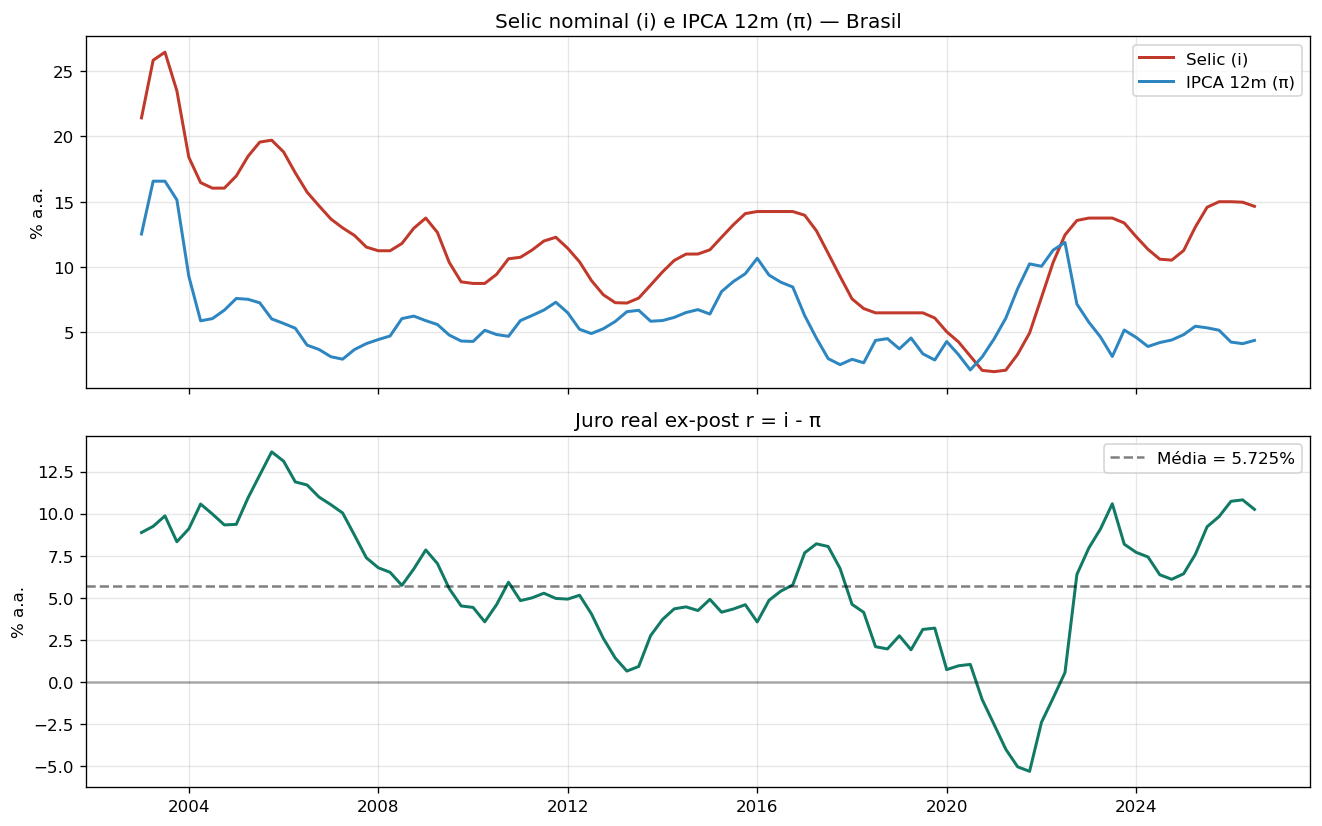
\includegraphics[width=\textwidth]{fig_fisher_lr.png}
\caption{Selic e IPCA 12m (painel superior) e juro real ex-post
$r = i - \pi$ (painel inferior), 2003 a 2026.}
\label{fig:fisher}
\end{figure}

\subsection{Neutralidade da moeda (VAR)}\label{sec:neutro}

Para testar se $r$ é independente de $i$ no longo prazo, estimo um VAR
em $(\pi, i)$ (exclui-se $r$ do VAR porque $r = i - \pi$ é identidade
linear) e infiro a resposta de $r$ pela identidade aplicada às trajetórias
de resposta. Lags escolhidos por AIC: 4.

\begin{table}[H]
\centering
\small
\begin{tabular}{lc}
\toprule
Teste & Valor \\
\midrule
Rank de cointegração (Johansen) & 2 \\
Granger $i \to \pi$ (menor $p$) & $0{,}000$ \\
Granger $\pi \to i$ (menor $p$) & $0{,}001$ \\
Resposta de $\pi$ a +1pp em $i$ (20 tri) & $+0{,}016$ \\
Resposta de $r$ (inferida) a +1pp em $i$ (20 tri) & $+0{,}131$ \\
\% variância de $\pi$ por choques em $i$ (20 tri) & $26{,}6\%$ \\
\bottomrule
\end{tabular}
\caption{VAR $(\pi, i)$ e teste de neutralidade.}
\label{tab:neutro}
\end{table}

A IRF revela um padrão rico: nos primeiros 2 ou 3 trimestres após um
choque de alta de Selic, a inflação \emph{sobe} (efeito neofisheriano
de curto prazo); do 4º ao 10º trimestre a inflação cai (canal
convencional); e no longo prazo converge para próximo de zero. Este é o
\emph{price puzzle} clássico de VARs brasileiros, bem documentado na
literatura (por exemplo, Minella et al., 2003 \cite{minella2003}). A
neutralidade estrita falha ($r$ varia $+0{,}13$ a um choque em $i$),
mas a magnitude é baixa. A política monetária explica $26{,}6\%$ da
variância de $\pi$: moderado, nem desprezível nem dominante.

A causalidade bidirecional (ambos os sentidos significativos) é
particularmente relevante: contraria a hipótese ``BC reage mas Selic
não causa inflação'' que seria mais favorável à tese neofisheriana pura.

% =====================================================================
\section{Pass-through cambial}\label{sec:cambio}
% =====================================================================

A proposta ALR prevê usar reservas (US\$ 350 bi) para neutralizar
depreciações cambiais decorrentes do corte de juros. A eficácia depende
do pass-through brasileiro. Estimo a regressão
\[
\Delta \pi^{livres}_t = \alpha + \sum_{k=0}^{2} \gamma_k \Delta e_{t-k}
                       + \beta \pi^{livres}_{t-1} + \varepsilon_t
\]
usando o IPCA livres (mais sensível ao câmbio do que o cheio, que
inclui administrados). A Tabela~\ref{tab:cambio} reporta os resultados.

\begin{table}[H]
\centering
\small
\begin{tabular}{lcc}
\toprule
Coeficiente & Valor & $p$-valor \\
\midrule
$\gamma_0$ (contemporâneo) & $-0{,}003$ & $0{,}770$ \\
$\gamma_1$ (lag 1) & $-0{,}001$ & $0{,}963$ \\
$\gamma_2$ (lag 2) & $+0{,}014$ & $0{,}210$ \\
$\pi^{livres}_{t-1}$ & $-0{,}095$ & $0{,}027$ \\
\midrule
Pass-through acumulado ($\sum \gamma$) & $\mathbf{+0{,}010}$ & \\
Reação cambial a +1pp Selic (8 tri, VAR) & $-7{,}22\%$ & \\
Canal indireto Selic $\to$ Câmbio $\to \pi$ & $-0{,}075$ p.p. & \\
\bottomrule
\end{tabular}
\caption{Pass-through cambial e canal indireto.}
\label{tab:cambio}
\end{table}

O pass-through brasileiro é excepcionalmente baixo (1\% acumulado), contra
5 a 15\% na literatura (BCB, Minella et al., 2003 \cite{minella2003}) e
10 a 30\% em emergentes típicos. Isso tem duas implicações para a proposta
ALR:

(1) O canal cambial contribui com apenas $8{,}5\%$ do efeito total da
Selic sobre a inflação. Os outros $91{,}5\%$ vêm de canais diretos
(demanda, expectativas, inércia).

(2) As reservas internacionais são mais que suficientes para neutralizar
o canal cambial, mas isso é quase irrelevante dado que o canal é
tão fraco. A proposta ALR dá importância a um elemento operacional
(intervenção com reservas) cujo efeito marginal sobre o resultado final
é pequeno.

% =====================================================================
\section{Posicionamento estrutural do Brasil}\label{sec:macro}
% =====================================================================

A teoria macroeconômica aplicada (Fisher, TFPL) foi desenvolvida assumindo
um ``país genérico'' tipicamente próximo dos EUA. Para avaliar se a
proposta ALR é Brasil-específica ou generalizável, posiciono o Brasil
contra 31 países em quatro eixos estruturais: produção/comércio, finanças
globais, social e institucional.

A Tabela~\ref{tab:ranking} sintetiza a posição do Brasil (entre 31 países).

\begin{table}[H]
\centering
\small
\begin{tabular}{lcc}
\toprule
Dimensão & Valor Brasil & Posição (31 países) \\
\midrule
PIB per capita PPP (USD) & $19.652$ & $24/31$ \\
ECI (complexidade, Hausmann) & $+0{,}15$ & $20/31$ \\
Abertura comercial (\% PIB) & $35{,}6$ & $27/29$ (quase o mais fechado) \\
Commodities (\% exp.) & $70{,}0$ & $26/31$ (alta dependência) \\
Gini & $50{,}3$ & $28/30$ (3º mais desigual) \\
Dívida/PIB (\%) & $81{,}9$ & $14/19$ \\
Reservas/PIB (\%) & $15{,}1$ & $14/31$ \\
Dívida em moeda local (\%) & $95$ & top (banda alta) \\
CBI (Dincer-Eichengreen) & $0{,}70$ & média-alta \\
\bottomrule
\end{tabular}
\caption{Posicionamento estrutural do Brasil (dados mais recentes, 2024).
Fontes: World Bank WDI, Atlas Harvard, BIS, Dincer-Eichengreen.}
\label{tab:ranking}
\end{table}

\begin{figure}[H]
\centering
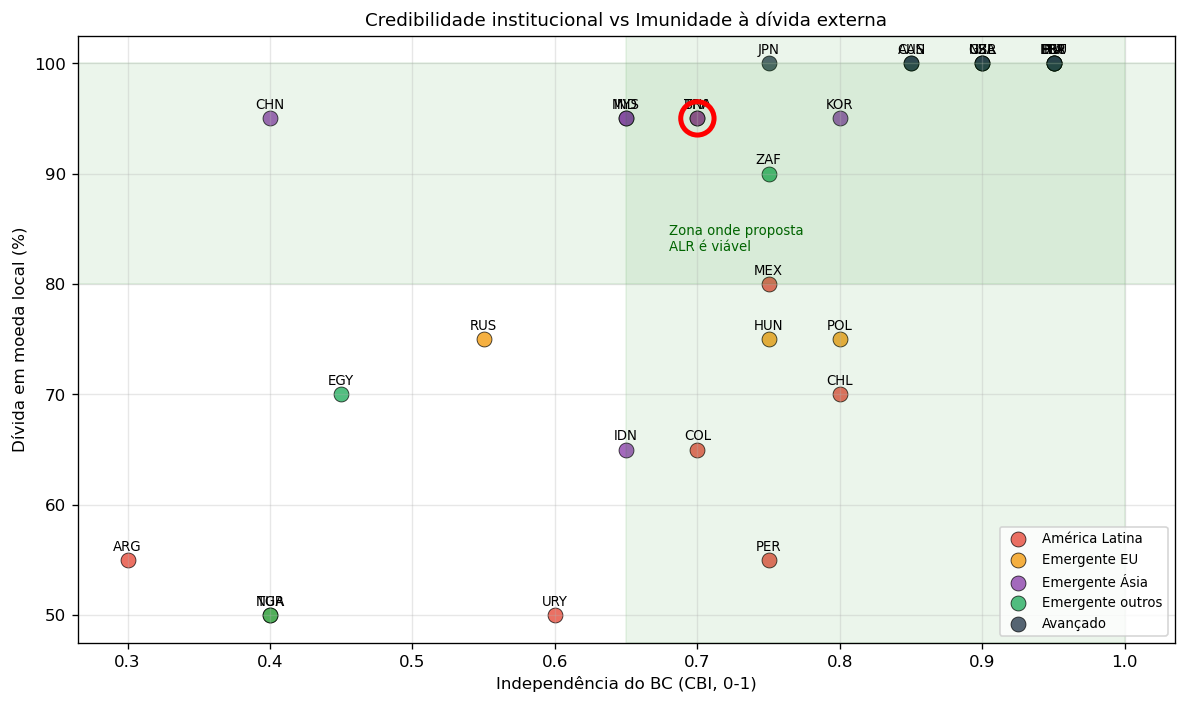
\includegraphics[width=0.95\textwidth]{fig_macro_eixo4_institucional.png}
\caption{Independência do BC (CBI) vs dívida em moeda local. A zona
sombreada em verde é onde a proposta ALR é teoricamente viável
(CBI > 0{,}65 E dívida local > 80\%). Brasil pertence a esse cluster.}
\label{fig:macro_inst}
\end{figure}

Dos 31 países, 15 satisfazem ambos os critérios (CBI alto E dívida local
alta), mas apenas 4 emergentes: \textbf{Brasil, Tailândia, Coreia do
Sul, África do Sul}. Turquia (CBI = 0{,}40), Argentina (0{,}30), Nigéria
(0{,}40) não têm a arquitetura institucional necessária.

A leitura substantiva é que o Brasil está em um espaço estrutural raro.
Tem a proteção institucional que torna a proposta ALR
teoricamente viável (algo que poucos emergentes têm), mas tem também as
vulnerabilidades estruturais (dependência de commodities,
Gini alto, economia fechada) que tornam o custo de errar maior do que
seria em Chile, Coreia ou Polônia. ALR argumenta sobre a arquitetura
monetária e fiscal, mas subestima que os efeitos distribucionais,
cambiais e setoriais vão operar sobre uma estrutura desfavorável.

% =====================================================================
\section{Simulação contrafactual da proposta ALR}\label{sec:sim}
% =====================================================================

Esta seção simula a proposta ALR (2026) no modelo macro reduzido calibrado
com os coeficientes estimados. A regra ALR é operacionalizada como:
\begin{itemize}[leftmargin=2em,topsep=0.3em]
  \item Transição (4 trimestres): Selic cai linearmente de 14{,}65\% a 7{,}5\%
  \item Regime permanente: $i_t = \max(\pi^*, \min(\pi^* + g_{pot} + 2, 7{,}5 + 0{,}3(\pi_t - \pi^*)))$
  \item Reancoragem: $\mathbb{E}\pi_t = (1-w_t)\pi_t + w_t \pi^*$, com $w_t$ subindo
    gradualmente até 0{,}5
\end{itemize}

\paragraph{Correção técnica necessária.} As estimações originais produziram
$\beta_b + \beta_f = 1{,}22 > 1$, o que gera inflação explosiva no longo
prazo. Para a simulação, normalizo para $\beta_b + \beta_f = 1$ (verticalidade
de longo prazo, padrão em Galí, 2015 \cite{gali2015}), preservando a proporção
relativa ($\beta_b = 0{,}575, \beta_f = 0{,}425$). Esta é uma limitação
metodológica a ser declarada: a normalização é teoricamente justificável
mas não é inocente.

Comparo cinco cenários: Taylor baseline (estimado), Taylor ortodoxa
($\phi_\pi = 2$, $\phi_y = 0{,}5$), ALR puro (sem reancoragem), ALR +
reancoragem, e ALR completo (reancoragem + intervenção cambial se
depreciação > 15\%).

\begin{figure}[H]
\centering
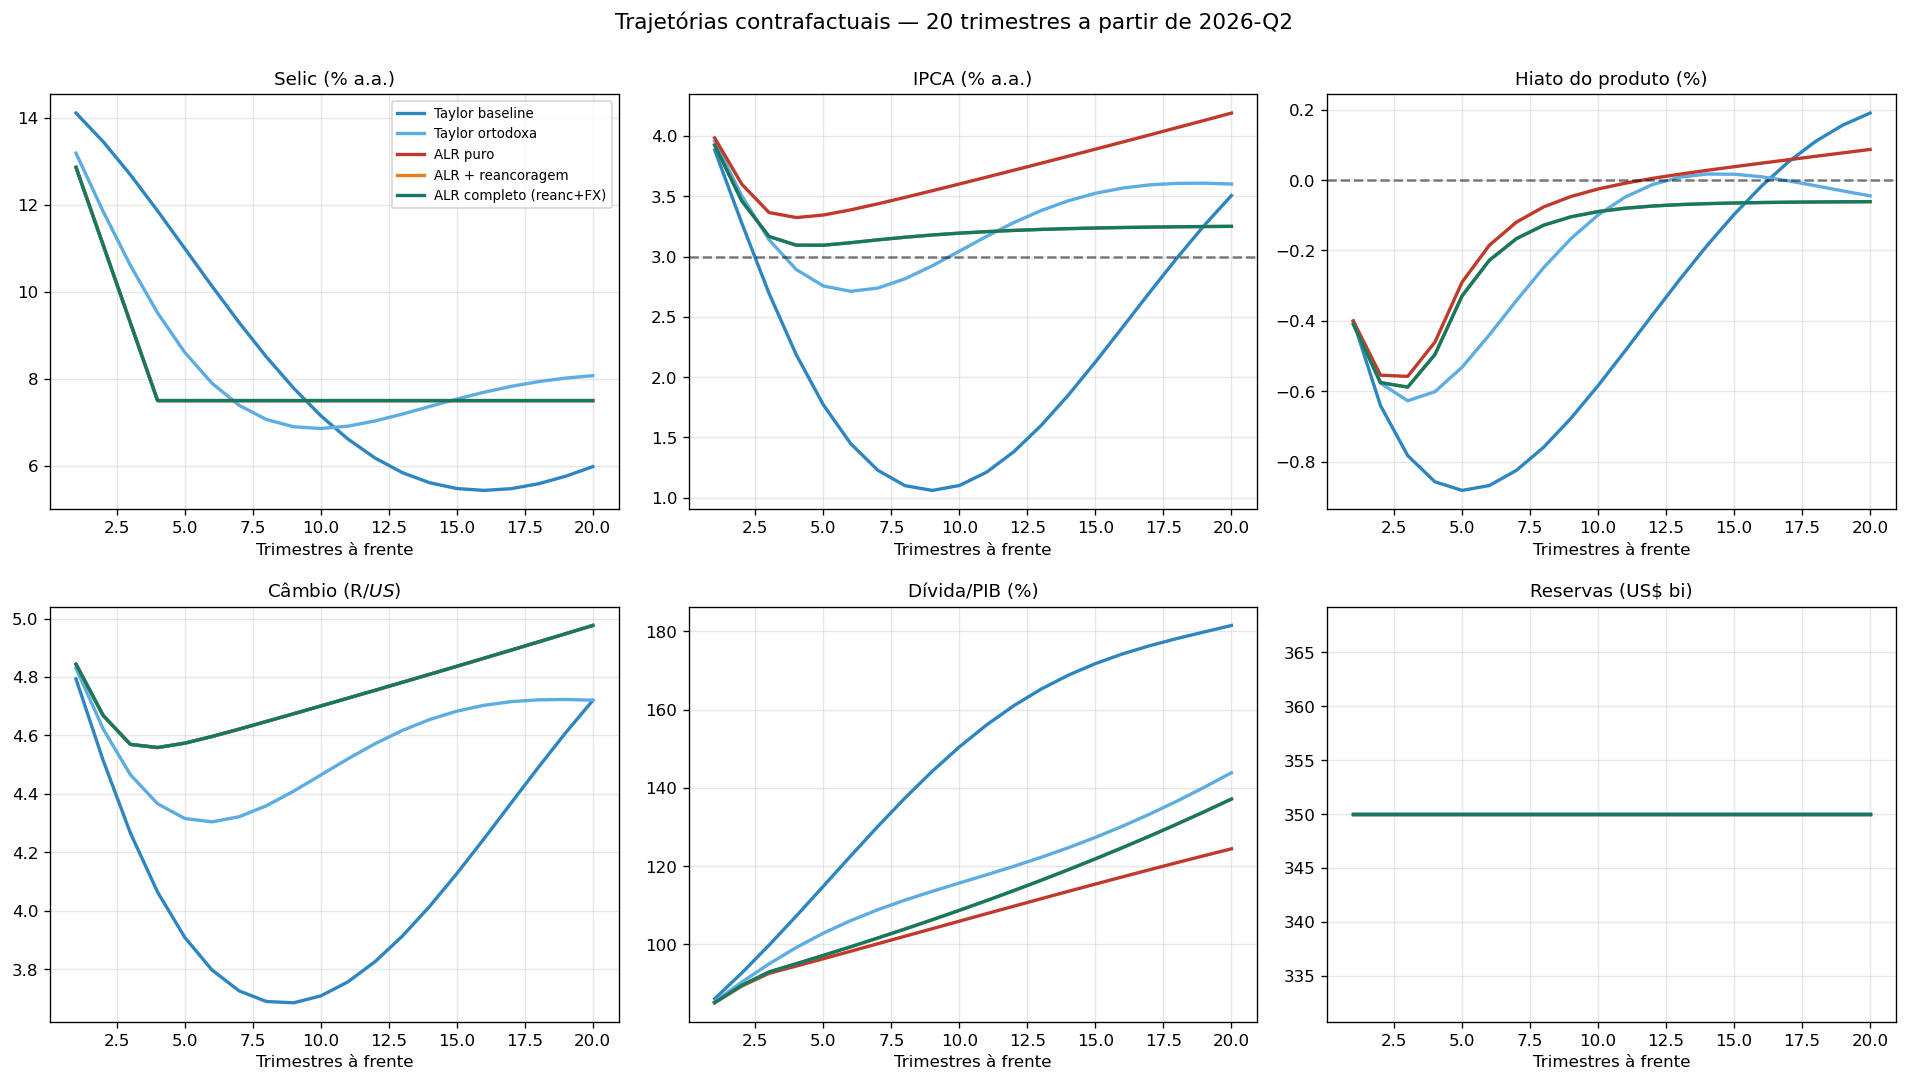
\includegraphics[width=\textwidth]{fig_cenarios_trajetorias.png}
\caption{Trajetórias contrafactuais de Selic, inflação, hiato, câmbio,
dívida e reservas sob cinco regras de política monetária (20 trimestres
a partir de 2026-Q2).}
\label{fig:cenarios}
\end{figure}

\begin{table}[H]
\centering
\small
\begin{tabular}{lcccc}
\toprule
Cenário & $\pi_{20}$ (\%) & $i_{20}$ (\%) & $b_{20}$ (\%) & $\Delta b$ vs Taylor (p.p.) \\
\midrule
Taylor baseline & $3{,}51$ & $5{,}98$ & $181{,}5$ & --- \\
Taylor ortodoxa & $3{,}60$ & $8{,}07$ & $143{,}9$ & $-37{,}6$ \\
ALR puro & $4{,}19$ & $7{,}50$ & $124{,}4$ & $-57{,}1$ \\
ALR + reancoragem & $3{,}25$ & $7{,}50$ & $137{,}2$ & $-44{,}4$ \\
ALR completo & $3{,}25$ & $7{,}50$ & $137{,}2$ & $-44{,}4$ \\
\bottomrule
\end{tabular}
\caption{Resultados da simulação em 20 trimestres (2026-Q2 a 2031-Q2),
determinística (sem choques).}
\label{tab:sim}
\end{table}

Três leituras-chave:

Primeiro, o baseline Taylor leva a dívida para $181\%$ do PIB em 5 anos,
uma trajetória insustentável. Esse é precisamente o cenário contra
o qual a proposta ALR compara, e dá fundamento à urgência.

Segundo, a proposta ALR completa (com reancoragem) entrega $\pi = 3{,}25\%$
(próximo da meta) e dívida de $137\%$ do PIB (vs $181\%$ baseline),
economia de $44$ p.p.\ de dívida em 5 anos. Em valores absolutos (PIB
$\sim$ R\$ 13 tri), são $\sim$ R\$ $5{,}7$ tri de dívida nominal evitada.

Terceiro, o ganho fiscal depende criticamente da reancoragem: ALR puro
(sem reancoragem) entrega $\pi = 4{,}19\%$ (acima da meta) e dívida
$124\%$, ainda melhor que baseline, mas com mais inflação.

A análise de sensibilidade (Tabela~\ref{tab:sens}) revela que cortes
mais rápidos produzem mais economia fiscal, contrariando a intuição de
gradualismo.

\begin{table}[H]
\centering
\small
\begin{tabular}{lccc}
\toprule
Velocidade do corte & $\pi_{20}$ (\%) & $b_{20}$ (\%) & Econ. serviço (\% PIB) \\
\midrule
6 meses (2 tri), choque & $3{,}27$ & $120{,}6$ & $+1{,}27$ \\
12 meses (4 tri), ALR & $3{,}25$ & $137{,}2$ & $-0{,}47$ \\
18 meses (6 tri) & $3{,}23$ & $154{,}3$ & $-2{,}46$ \\
24 meses (8 tri), gradual & $3{,}21$ & $173{,}0$ & $-4{,}82$ \\
\bottomrule
\end{tabular}
\caption{Sensibilidade à velocidade do corte da Selic. A inflação é
praticamente insensível, mas a dívida acumula o custo do atraso.}
\label{tab:sens}
\end{table}

% =====================================================================
\section{Discussão}\label{sec:disc}
% =====================================================================

A Tabela~\ref{tab:conclusao} sintetiza a conclusão de cada proposição do
argumento ALR.

\begin{table}[H]
\centering
\small
\begin{tabular}{lcl}
\toprule
Proposição & Status & Mecanismo empírico \\
\midrule
1. Aritmética fiscal grave & \textbf{Sustentada} & $p^* = 7{,}1\%$ vs $p = 1{,}06\%$ \\
2. Phillips plana & \textbf{Sustentada} & $\kappa = 0{,}04$ (n.s.) \\
3. IS fraca & Sustentada & $\sigma = 0{,}06$ (p=0,07) \\
4. Fisher de LP ($\beta > 0$) & Parcial & $\beta_{OLS}>0$, Johansen $<0$ \\
5. Fisher puro ($\beta = 1$) & \textbf{Rejeitada} & $p < 0{,}001$ \\
6. Neutralidade estrita & Parcial & resp. $r = +0{,}13$ em 20t \\
7. Pass-through baixo & \textbf{Sustentada} & 1\% acumulado \\
8. Arquitetura institucional & \textbf{Sustentada} & dívida 95\% local, CBI 0{,}70 \\
9. Proposta viável no modelo & Sim, com condição & requer reancoragem \\
\bottomrule
\end{tabular}
\caption{Conclusão consolidada das proposições de ALR à luz dos dados
brasileiros 2003 a 2026.}
\label{tab:conclusao}
\end{table}

\paragraph{O que o paper sustenta.} A tese fiscal é inescapável: a dívida
cresce na trajetória atual, e o gap primário é grande. A tese da Phillips
plana é corroborada: o hiato praticamente não desloca a inflação brasileira.
O pass-through cambial baixo torna o canal cambial quase irrelevante,
reservas sobram para neutralizá-lo. A arquitetura institucional brasileira
coloca o país em um clube pequeno de emergentes onde essa proposta pode
ser testada. E a simulação calibrada entrega ganho fiscal expressivo sem
descontrole inflacionário, desde que a reancoragem funcione.

\paragraph{O que o paper não sustenta.} Fisher puro ($\beta = 1$) é
rejeitado com folga; a leitura literal ``cortar Selic para 7{,}5\%
leva $\pi$ para 5\%'' não se sustenta. A neutralidade estrita falha
marginalmente ($r$ varia a choques em $i$). A causalidade $i \to \pi$
é significativa (Selic efetivamente causa inflação), o que contraria a
leitura ``BC reage mas não causa'' que seria mais favorável à tese
neofisheriana pura. O \emph{price puzzle} de curto prazo (inflação sobe
antes de cair) complica a narrativa política da proposta.

\paragraph{O ponto cego estrutural.} ALR fala da arquitetura monetária e
fiscal (onde o Brasil está relativamente bem posicionado) mas subestima
a estrutura produtiva e social (onde o Brasil é vulnerável). Em um país
com pauta 70\% commodities, Gini de 50 e economia fechada, o custo de
errar a transição é muito maior do que em Chile, Coreia ou Polônia.
Essa dimensão não aparece no argumento de ALR, e deveria.

\paragraph{Limitações.} O modelo é em forma reduzida, com expectativas
adaptativas na simulação. A normalização $\beta_b + \beta_f = 1$ é
uma correção teórica que mascara um fato empírico (as estimativas somam
$1{,}22$). O tratamento do primário como exógeno ignora uma possível
\emph{fiscal reaction function} (Bohn, 1998 \cite{bohn1998}). O filtro
HP tem \emph{end-point bias} conhecido. O pass-through pode ser
subestimado pela agregação em livres cheios. A reancoragem é modelada
mas não demonstrada. Extensões naturais: GMM com instrumentos para
$\mathbb{E}\pi$, DSGE com expectativas racionais (estilo SAMBA do BCB),
decomposição da dívida por indexador (LFT vs prefixados vs IPCA),
análise de episódios análogos internacionais (Turquia 2021 a 2023, Argentina
2024, Rússia 2022).

% =====================================================================
\section{Salvaguardas em cenário desfavorável}\label{sec:salvaguardas}
% =====================================================================

A simulação da Seção~\ref{sec:sim} é determinística e assume que a
reancoragem institucional funciona. A Seção~\ref{sec:disc} apontou quatro
limitações estruturais que podem materializar um cenário mais adverso do
que o modelado. Esta seção propõe um conjunto de salvaguardas que podem
reduzir o custo da proposta em caso de execução imperfeita, inspiradas
em arranjos adotados em outras experiências de regime monetário e em
mecanismos de política fiscal contracíclica.

Seis salvaguardas se destacam.

\paragraph{1. Cláusula de reversão monetária (circuit breaker).} Se a
inflação acumulada em 12 meses superar a meta em mais de dois pontos
percentuais por dois trimestres consecutivos, a Selic retorna
progressivamente para um patamar intermediário pré-definido (por exemplo,
10\%), até que a inflação volte a convergir. Isso elimina o risco de
captura ideológica do arranjo e sinaliza ao mercado que o experimento
é reversível sem ruptura institucional.

\paragraph{2. Reserva de defesa cambial com protocolo automático.} Do
estoque de reservas, uma parcela (por exemplo, US\$ 100 bi) é designada
como ``reserva de defesa cambial'' com uso vinculado a regra pública.
Intervenção só se ativa se a depreciação acumulada superar 20\% em janela
de 12 meses. Isso evita gasto discricionário das reservas e torna a
intervenção previsível, reduzindo o incentivo ao ataque especulativo.

\paragraph{3. Trava de composição da dívida.} Durante a transição, o
Tesouro reduz emissão nova de LFTs e amplia a participação de prefixados
e NTN-B. A dívida pós-fixada em Selic funciona como amplificador do custo
quando a política monetária é apertada, e como atenuador quando é
afrouxada. Reduzir a participação de LFTs durante a janela de corte
diminui a velocidade de propagação do ganho fiscal no curto prazo, mas
protege o Tesouro caso a Selic precise voltar a subir (salvaguarda 1).

\paragraph{4. Mecanismo de compensação distributiva.} A proposta ALR
reduz o estoque de dívida pública, cujos títulos estão concentrados nos
decis mais ricos da distribuição de renda. Para evitar efeito regressivo,
uma fração da economia de serviço da dívida (por exemplo, 20\%) é
vinculada a transferências condicionais para os dois decis inferiores.
Isso neutraliza a crítica distributiva e ancora politicamente a
sustentação da reforma.

\paragraph{5. Metas intermediárias com publicação trimestral obrigatória
pelo CFMN.} O arranjo institucional proposto por ALR só gera reancoragem
se produzir transparência verificável. Publicação trimestral dos desvios
acumulados de inflação, câmbio e dívida/PIB frente à trajetória prevista,
com explicação técnica e eventual acionamento dos circuit breakers, cria
a âncora comportamental de expectativas que o modelo assume sem demonstrar.

\paragraph{6. Agenda estrutural paralela.} O pass-through cambial baixo
e a curva de Phillips plana que fundamentam a viabilidade da proposta
são sintomas de uma economia com crédito direcionado, indexação
disseminada, informalidade elevada e baixa complexidade exportadora.
Esses mesmos traços amplificam o custo de erro na transição. Uma agenda
estrutural paralela, de desindexação, abertura comercial gradual e
sofisticação da pauta exportadora, não é condição necessária para a
proposta funcionar no horizonte de cinco anos, mas é condição necessária
para que o próprio regime sobreviva a choques futuros.

Nenhuma dessas salvaguardas é inédita, cada uma tem precedente em
experiências internacionais (Chile, Nova Zelândia, Israel, Coreia do
Sul). O ponto é que elas transformam a proposta ALR de uma aposta
institucional em um desenho institucional mais robusto, capaz de operar
em cenários que o modelo determinístico da Seção~\ref{sec:sim} não captura.

% =====================================================================
\section{Conclusão}\label{sec:concl}
% =====================================================================

Os argumentos que André Lara Resende construiu entre 2017 e 2026 foram
submetidos a sete blocos empíricos. Do ponto de vista da aritmética
fiscal, o diagnóstico de ALR se confirma e se agrava. O superávit
primário necessário para estabilizar a relação dívida/PIB subiu de
5,1\% em 2017 para 7,1\% em 2026, enquanto o Brasil entrega pouco mais
de 1\%. A tese de que a curva de Phillips brasileira é quase horizontal
também se sustenta, com o coeficiente do hiato pequeno e não
significativo, e a transmissão da taxa de juros para a demanda
mostra-se igualmente fraca. Nesses dois pontos, a leitura de ALR é
fiel ao que os dados mostram.

Já o neofisherianismo, que sustenta a proposta de 2026, encontra apoio
parcial. Inflação e Selic efetivamente cointegram no longo prazo, e o
sinal da relação é positivo como prevê a identidade de Fisher. Mas o
coeficiente estimado está bem abaixo de um, de modo que a leitura mais
radical, segundo a qual cortar a Selic levaria a inflação mecanicamente
para baixo, não encontra base empírica no Brasil. O que os dados
mostram é um movimento conjunto de longo prazo, não uma relação um
para um.

A simulação contrafactual indica que a proposta pode funcionar no
modelo calibrado, produzindo ganho fiscal relevante sem descontrole
inflacionário, contanto que haja reancoragem institucional crível. Esse
ponto é central e não deve ser lido como detalhe técnico. Sem a
reancoragem, a inflação se mantém acima da meta ao longo de todo o
horizonte simulado, enquanto com ela converge para perto de 3\%. O
CFMN proposto por ALR busca precisamente oferecer esse mecanismo de
ancoragem, e a viabilidade da proposta depende em boa medida de o
arranjo institucional entregar o que promete. As salvaguardas discutidas
na Seção~\ref{sec:salvaguardas} tornam o arranjo mais robusto em
cenários que fogem ao previsto.

Há um elemento adicional que o texto de ALR não enfatiza mas que o
posicionamento estrutural do Brasil torna evidente. A proposta repousa
sobre uma arquitetura financeira bastante favorável, com dívida quase
inteiramente em moeda local, reservas internacionais superiores a 15\%
do PIB, câmbio flutuante e banco central com credibilidade institucional
razoável. Esse conjunto é raro entre emergentes, e Turquia, Argentina
e Nigéria, por exemplo, não têm nada parecido. Nesse sentido, o Brasil
está entre os poucos países onde uma proposta como essa pode ser
considerada com seriedade. Por outro lado, a estrutura produtiva e
social, com forte dependência de commodities, economia relativamente
fechada e desigualdade elevada, torna o custo de um erro de transição
desproporcionalmente alto. ALR trata com cuidado a arquitetura monetária
e fiscal, mas pouco discute esse pano de fundo estrutural.

O que emerge deste trabalho, portanto, não é um veredito sobre
heterodoxia ou ortodoxia, nem um endosso ou rejeição da proposta. É
uma leitura mais sóbria. A aritmética fiscal confirma a urgência do
problema, a mecânica monetária brasileira é de fato fraca, o
neofisherianismo oferece uma direção correta embora com magnitudes
mais modestas do que a versão forte da tese sugere, a proposta
operacional é tecnicamente viável no modelo e está longe de ser
absurda, e sua execução efetiva depende de condições institucionais
e estruturais específicas do Brasil que precisam ser reconhecidas
honestamente. Se o paper contribui com algo, é com a sugestão de
que esse debate deveria se dar nesses termos, e não entre polos
ideológicos antagônicos.

\subsection*{Nota sobre métodos e ferramentas}

Este trabalho foi concebido, conduzido e redigido por mim. No processo,
utilizei um assistente de inteligência artificial (Claude, da Anthropic)
como ferramenta de apoio para acelerar a escrita do código de coleta
e tratamento de dados (APIs BACEN/SGS, Olinda, SIDRA, World Bank),
depurar a integração entre bibliotecas econométricas (statsmodels,
pandas), discutir escolhas de especificação e acelerar a formatação
deste documento em \LaTeX. Todas as decisões de modelagem, a
interpretação dos resultados e a responsabilidade pelo conteúdo são
exclusivamente minhas. O código fonte completo, dados consolidados,
sete notebooks reprodutíveis (um por bloco empírico) e um notebook
consolidado final estão disponíveis em
\url{https://github.com/walterCNeto/PoliticaMonetariaALR}.

% =====================================================================
\renewcommand{\refname}{Referências}
\begin{thebibliography}{99}

\bibitem{bohn1998}
Bohn, H. (1998). The behavior of U.S. public debt and deficits.
\emph{Quarterly Journal of Economics}, 113(3), 949 a 963.

\bibitem{cochrane2011}
Cochrane, J. H. (2011). Inflation and debt. \emph{National Affairs}, n.~9,
outono.

\bibitem{cochrane2023}
Cochrane, J. H. (2023). \emph{The Fiscal Theory of the Price Level}.
Princeton: Princeton University Press.

\bibitem{cochrane2026}
Cochrane, J. H. (2026). ``Reasons to Lower Rates'' e ``More on Lower
Rates''. \emph{The Grumpy Economist}, Substack, setembro.

\bibitem{dincer2014}
Dincer, N. N. e Eichengreen, B. (2014). Central bank transparency and
independence: updates and new measures. \emph{International Journal of
Central Banking}, 10(1), 189 a 253.

\bibitem{du_schreger2016}
Du, W. e Schreger, J. (2016). Local currency sovereign risk.
\emph{Journal of Finance}, 71(3), 1027 a 1070.

\bibitem{gali2015}
Galí, J. (2015). \emph{Monetary policy, inflation, and the business cycle:
An introduction to the New Keynesian framework and its applications}. 2ª
ed. Princeton University Press.

\bibitem{hausmann2014}
Hausmann, R., Hidalgo, C.~A. et al. (2014). \emph{The Atlas of Economic
Complexity: Mapping Paths to Prosperity}. MIT Press.

\bibitem{hp1997}
Hodrick, R. J. e Prescott, E. C. (1997). Postwar U.S. business cycles:
An empirical investigation. \emph{Journal of Money, Credit and Banking},
29(1), 1 a 16.

\bibitem{johansen1991}
Johansen, S. (1991). Estimation and hypothesis testing of cointegration
vectors in Gaussian vector autoregressive models. \emph{Econometrica},
59(6), 1551 a 1580.

\bibitem{kuttner2010}
Kuttner, K. e Robinson, T. (2010). Understanding the flattening Phillips
curve. \emph{North American Journal of Economics and Finance}, 21(2),
110 a 125.

\bibitem{lararesende2017}
Lara Resende, A. (2017). Juros e conservadorismo intelectual.
\emph{Valor Econômico}, janeiro de 2017.

\bibitem{lararesende2026}
Lara Resende, A. (2026). Eu Acuso: uma proposta para eliminar os juros
absurdos. \emph{Substack ``Um Cético Esperançoso''}, 25 de setembro de 2026.

\bibitem{minella2003}
Minella, A., Freitas, P. S., Goldfajn, I. e Muinhos, M. K. (2003).
Inflation targeting in Brazil: Constructing credibility under exchange
rate volatility. \emph{Journal of International Money and Finance}, 22(7),
1015 a 1040.

\bibitem{newey1987}
Newey, W. K. e West, K. D. (1987). A simple, positive semi-definite,
heteroskedasticity and autocorrelation consistent covariance matrix.
\emph{Econometrica}, 55(3), 703 a 708.

\bibitem{sims1980}
Sims, C. A. (1980). Macroeconomics and reality. \emph{Econometrica},
48(1), 1 a 48.

\bibitem{taylor1993}
Taylor, J. B. (1993). Discretion versus policy rules in practice.
\emph{Carnegie-Rochester Conference Series on Public Policy}, 39,
195 a 214.

\end{thebibliography}

\end{document}
